\documentclass{beamer}

\usepackage{cmap}
\usepackage{mathtext}
\usepackage[T2A]{fontenc}
\usepackage[utf8]{inputenc}
\usepackage[english,russian]{babel}
\usepackage{amsmath,amsfonts,amssymb,amsthm,mathtools}
\usepackage{listings}

\title{Physics of Light}

\usetheme{Berlin}

\begin{document}

\begin{frame}
  \titlepage
\end{frame}

\begin{frame}
  \frametitle{Проблема цвета}

  В прошлый раз вы могли видеть, что картинка была чёрно-белая, так как источник света испускал волны с одинаковой длиной волны.
\end{frame}

\begin{frame}
  \frametitle{Решение}

  Был реализован источник с тремя разными длинами волн (RGB), что позволило сделать картину опыта Юнга (а также и последующих) более эффектной.

  \begin{figure}[c]
    
\includegraphics[scale=0.3]{assets/colorYung.png}
  \end{figure}
\end{frame}

\begin{frame}
  \frametitle{Новый опыт!}

  Был проведён опыт с дифракционной решёткой. Для реализации был предложен вариант приближения отверстий квадратной сеткой, которая при достаточной плотности показывает достаточно правдоподобные результаты.
\end{frame}

\begin{frame}
  \frametitle{Результат}

  \begin{figure}[c]
    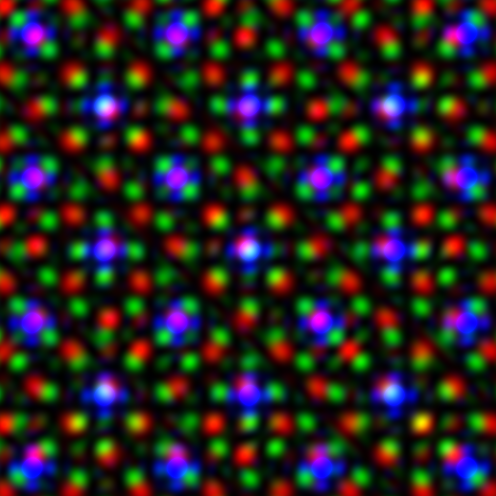
\includegraphics[scale=0.3]{assets/diffR1.png}
    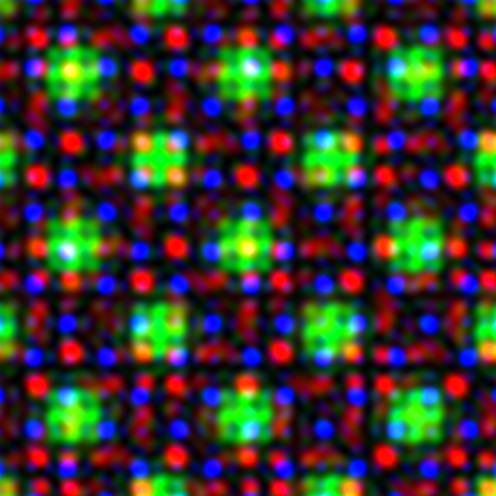
\includegraphics[scale=0.3]{assets/diffR2.png}
  \end{figure}
\end{frame}

\begin{frame}
  \frametitle{Новый опыт!}

  Был проведён опыт с линзой. 
  \begin{figure}[c]
    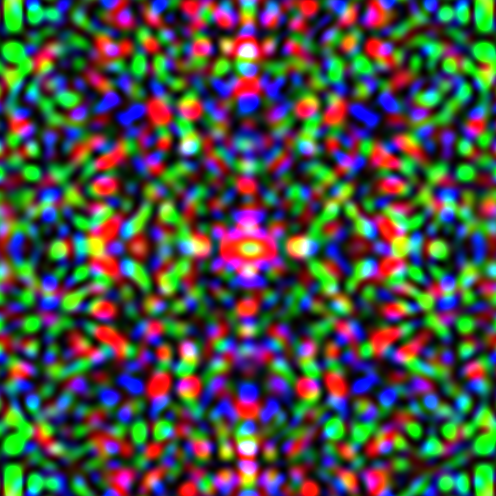
\includegraphics[scale=0.3]{assets/len1.png}
    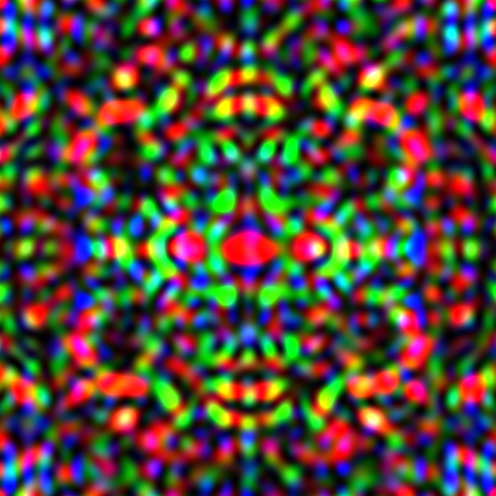
\includegraphics[scale=0.3]{assets/len2.png}
  \end{figure}
\end{frame}

\begin{frame}
  \frametitle{Поймать фокус}

  Нам удалось поймать фокус - сконцентрировали пучок света в центре, что дало более яркий картину по сравнению с остальными участками.

  \begin{figure}[c]
    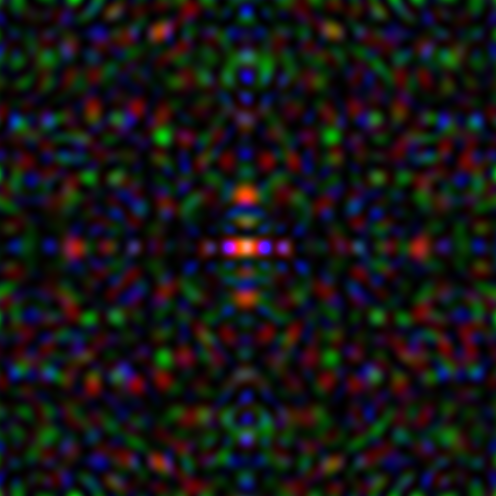
\includegraphics[scale=0.3]{assets/len3.png}
  \end{figure}
\end{frame}

\end{document}
